\documentclass[conference]{IEEEtran}
\IEEEoverridecommandlockouts

\usepackage{graphicx}
\usepackage{amsmath,amssymb}
\usepackage{booktabs}
\usepackage{stfloats}
\usepackage{flushend}
\usepackage[hidelinks]{hyperref}
\usepackage{url}

% Figures live next to this .tex file
\graphicspath{{./}}

\begin{document}

\title{Vision-Only Reactive Corridor Navigation\\
for a Quadruped: Reusing a Frozen\\
Velocity Policy with a Hard Passage Gate}

\author{\IEEEauthorblockN{Mohammadreza AhmadiTeshnizi, Patrik Per\v{c}ini\'{c} \quad (Team Ava)}
\IEEEauthorblockA{Robotics 2026, LIACS, Leiden University\\
Video: \url{https://github.com/teshnizi2/go2-ball-follower/blob/main/demo/go2_submission.mp4}\\
Code: \url{https://github.com/teshnizi2/go2-ball-follower}}}

\maketitle

\begin{abstract}
A simulated Unitree Go2 quadruped follows a moving red ball down a cluttered corridor
using only its head camera: no GPS, lidar, depth sensor, or map. The gait comes
from a frozen, pre-trained reinforcement-learning policy whose weights we never touch;
around it we build a colour tracker, a reactive gap-picking planner, and the corridor
generator. The policy accepts a sideways velocity command, but a controller that only
walks toward a target leaves that channel at zero, so the robot turns to move sideways,
like a car changing lanes. We switch the channel back on and add one rule: the robot may
not enter an obstacle row until aligned with the gap. A logged 150~s run is collision-free
at 0.64~m/s, on average 0.66~m from the ball, and a longer run reaches stage 17
collision-free. The ball passes straight through the obstacles, so the robot alone avoids
them.
\end{abstract}

\section{Introduction}
Most robots that move through cluttered spaces rely on rich sensing (lidar, depth
cameras, or motion capture) and a mapping-and-planning stack on top. We ask the opposite
question: how far can a four-legged robot get through a dense obstacle corridor with only
a single RGB camera on its head and a walking controller it did not train?

The robot chases a moving red ball, a stand-in for a goal to walk toward. The corridor is
five metres wide and packed with rows of obstacles whose gaps tighten with distance. The
walking comes from a frozen, pre-trained reinforcement-learning (RL) policy from the
RSL-RL framework~\cite{rudin}, used as a black box whose weights we never change; the ball
tracking is plain colour vision. The planner, the safety rules, the corridor generator,
and the dashboard are ours.

\textbf{Contribution.} The policy of Rudin et al.~\cite{rudin} is omnidirectional: its
command is a forward speed, a sideways speed, and a turn rate $(v_x, v_y, v_\omega)$. A
controller that only walks toward the ball sets the forward speed and turn rate and leaves
$v_y$ at zero, so the robot is non-holonomic and must turn, walk, and turn back to shift
sideways. We show that driving this unused sideways channel, together with a gate that
refuses to enter a gap before the body is aligned, lets an untrained walker thread a tight
corridor with no collisions at all. We did not find this combination, reusing the spare
command channel of a frozen policy purely for reactive single-camera avoidance, in the
literature we surveyed. Section~\ref{sec:results} quantifies how much each layer
contributes.

\section{Related Work}
\textbf{Learned legged locomotion.} RL has produced strong quadruped controllers in
simulation and on real hardware~\cite{hwangbo}, including blind walking over rough
terrain~\cite{lee} and policies that learn velocity commands in minutes~\cite{rudin}. We
treat one such policy as a black box mapping a velocity command to joint motion, and never
retrain it.

\textbf{Reactive navigation.} We build no map. The planner reads the next row of
obstacles, picks a gap, and steers to it with a pure-pursuit law~\cite{coulter} --- closer
to follow-the-gap and potential-field methods than to global planning, which suits a
low-sensing robot that must react fast.

\textbf{Tracking the ball.} The ball is found with an HSV colour mask and followed with
CamShift~\cite{bradski}, a light histogram tracker chosen over a neural detector to keep
the pipeline simple to inspect. The simulator is MuJoCo~\cite{mujoco}; the Go2 model is
from the MuJoCo Menagerie.

\section{System Design}
The system wraps three layers around the frozen walking policy (Fig.~\ref{fig:arch}). The
camera feeds a tracker, the tracker feeds a planner, the planner and a hard gate shape a
velocity command, and the frozen policy turns that command into a gait; only the robot's
base pose and proprioception flow back.

\begin{itemize}
\item \textbf{Perception} (\texttt{tracker.py}) finds the red ball with an HSV mask and
follows it with CamShift, re-detecting when confidence drops.
\item \textbf{Reactive planning} (\texttt{controller.py}, \texttt{main.py}) picks a gap
through the next row, commits to it, and converts it into a body-frame velocity command
including the sideways slide. Pure pursuit follows the path; a hard gate and a push-away
term are the safety net.
\item \textbf{Walking} (\texttt{low\_level.py}) is the frozen policy. It reads a
45-number observation plus the velocity command and outputs 12 joint targets at 50~Hz,
tracked by a PD loop at 500~Hz.
\end{itemize}

A separate corridor generator lays out the obstacle rows, ramps difficulty with distance,
and recycles passed rows to the front so the course never ends.

\begin{figure*}[!t]
\centering
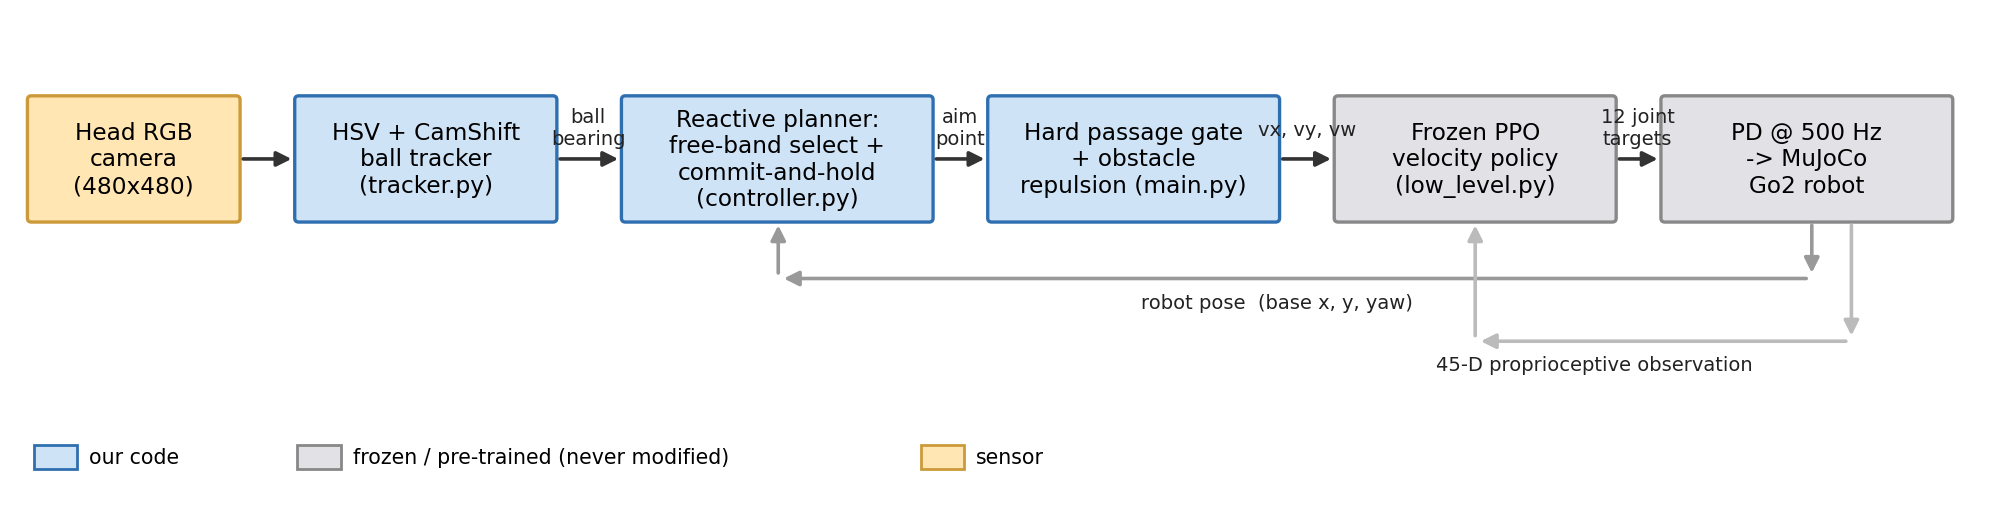
\includegraphics[width=\textwidth]{fig_architecture.png}
\caption{System pipeline. Blue blocks are code we wrote; grey blocks are the frozen,
pre-trained policy and the physics we never modify. The camera produces a ball bearing,
the planner produces an aim point, the gate shapes the velocity command
$(v_x, v_y, v_\omega)$, and only the robot's pose and a 45-D proprioceptive observation
feed back.}
\label{fig:arch}
\end{figure*}

\begin{figure}[htbp]
\centering
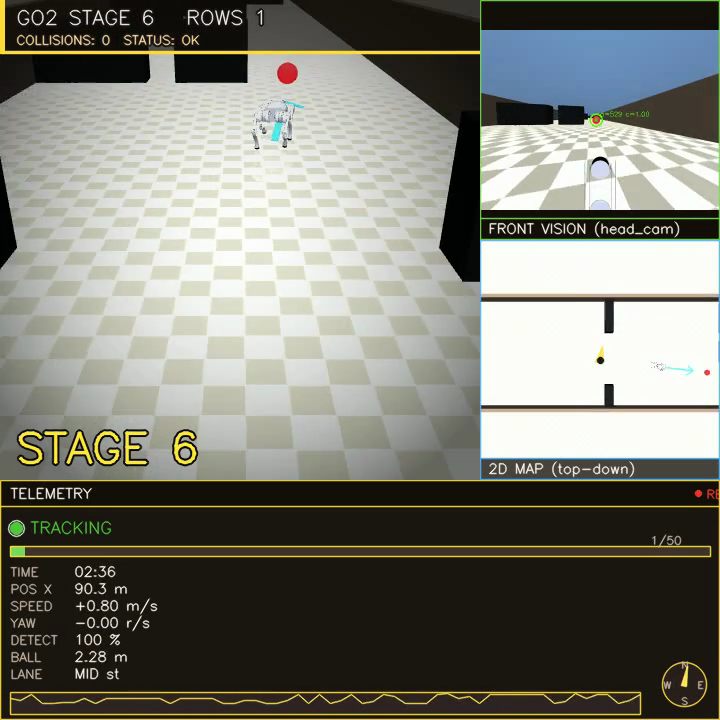
\includegraphics[width=\columnwidth]{fig_dashboard.png}
\caption{The $720\times720$ dashboard. Left: the chase view with the planned path drawn
on the floor and a halo on the obstacle being avoided. Top right: the robot's own head
camera with the tracked ball. Below it: a top-down map. The bottom strip shows speed,
range, detection confidence, a status light, and the stage.}
\label{fig:dash}
\end{figure}

\section{Implementation}

\subsection{Finding the ball}
Red wraps around the hue circle, so we use two HSV ranges and clean the mask with
morphology. The largest sensible blob seeds a box and a hue histogram, which CamShift
tracks frame to frame. Short occlusions are tolerated because the tracker coasts; a long
loss triggers a fresh detection. In simulation the ball's true position is known, so the
controller keeps chasing while the ball is hidden behind an obstacle.

\subsection{The planner and the gate}
For the next row, the planner inflates each obstacle by a safety margin (about the robot's
half-width plus slack), discards the blocked strips, and keeps the widest gap it can
reach. It aims at the centre of that gap, never an edge, and stays committed until the
robot is past the row; without commitment the ball can pull the robot back into an
obstacle it just cleared.

The gate (Fig.~\ref{fig:gate}) is the key mechanism. Until the robot is inside the chosen
band it may not pass the front of the row: its forward speed drops to zero at that line
while a strong sideways command slides it to the band centre, and only once aligned does
it move through. Forcing alignment before entry keeps the robot safe wherever the ball
leads it.

\begin{figure}[htbp]
\centering
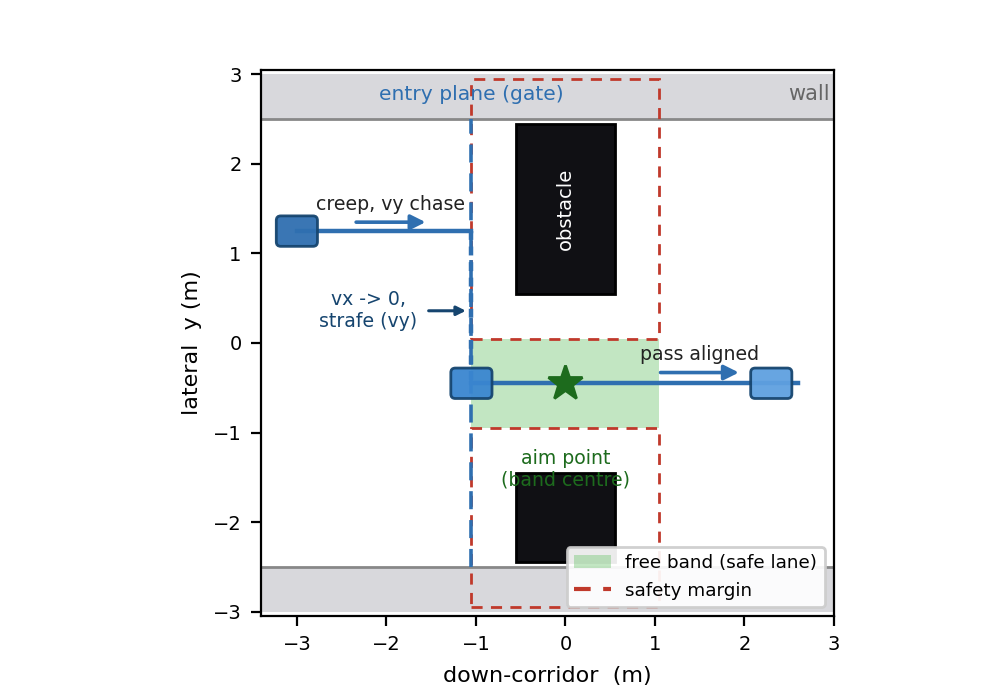
\includegraphics[width=\columnwidth]{fig_gate.png}
\caption{The free-band passage gate (top-down). Each obstacle is inflated by a safety
margin (dashed); the gap left between the inflated obstacles is the free band (green). The
robot creeps to the entry plane, drops $v_x$ to zero and strafes ($v_y$) to the band
centre, then passes through aligned. It never crosses the gate while misaligned.}
\label{fig:gate}
\end{figure}

\subsection{Turning the sideways channel back on}
\label{sec:vy}
We rotate the high-level command into the robot's own frame and feed its sideways part
into the policy's $v_y$ input, which our first version left at zero. With it on, the robot
steps directly into a wall-side gap instead of turning, walking, and turning back. A
push-away term nudges the body sideways near an obstacle edge as a backup. We cap forward
speed during sharp turns, where the frozen policy becomes unreliable, and a tripped robot
stands up where it fell rather than restarting the run.

\subsection{The corridor and the difficulty curve}
Every row leaves at least one lane wide enough for the robot; otherwise two wide obstacles
could split the corridor into impassable slivers and the planner would stall. Difficulty
grows with distance, not time (Fig.~\ref{fig:diff}): obstacles widen, the guaranteed lane
narrows toward a floor of 1.30~m, and the colour darkens, across 17 stages that climb and
then hold. The 1.30~m floor stays above the robot's 0.68~m width, so every row
is passable but the later ones leave little room. Passed rows recycle to the front, making
the corridor effectively endless, and the ball follows its own sine path straight
through the obstacles, so the robot can never trail a cleared route.

\begin{figure}[htbp]
\centering
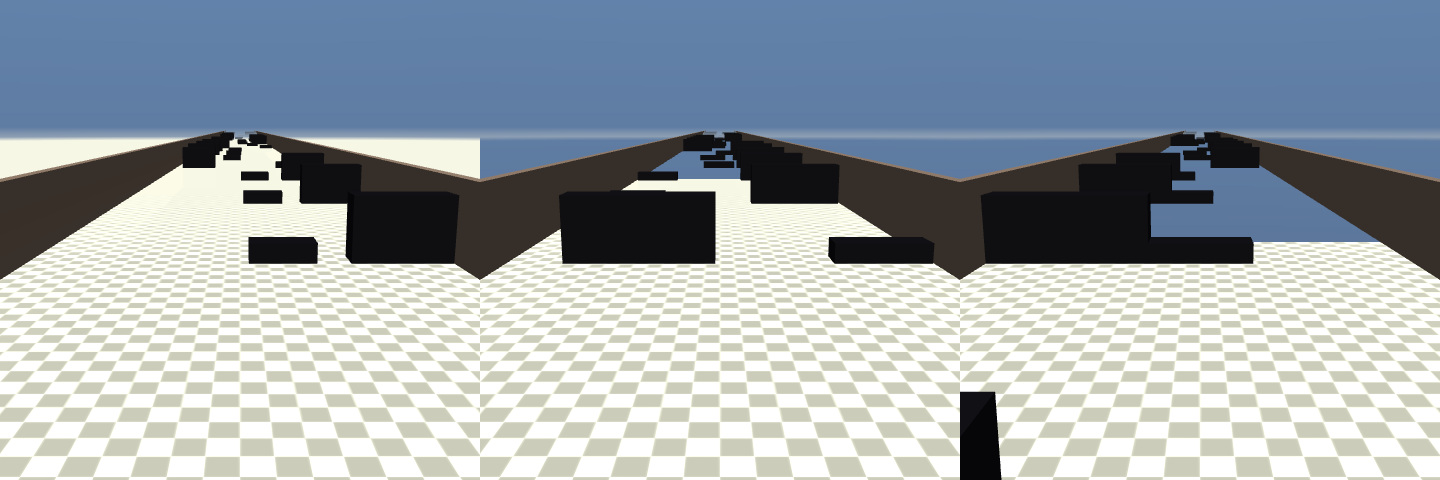
\includegraphics[width=\columnwidth]{fig_difficulty.png}
\caption{Difficulty as a function of distance, straight from the generator. Obstacles
widen while the guaranteed passage narrows to a 1.30~m floor, always above the robot's
0.68~m width (red line), so rows stay passable but tight. The blue staircase is the
difficulty stage (1 to 17).}
\label{fig:diff}
\end{figure}

\subsection{Control loop and runtime}
The control loop runs at 50~Hz and the physics at 500~Hz: the policy reads one observation
and emits one command every 20~ms while the PD loop and the contacts update ten times in
between. With the scene trimmed to the obstacles in use, the simulator steps at about
5{,}700~Hz on a laptop, several times faster than real time. A single OpenCV window
renders the full dashboard of Fig.~\ref{fig:dash}.

\section{Results}
\label{sec:results}
We evaluated the system headless, counting any contact between the robot and an obstacle or
wall as a failure. A logged 150~s run (seed 42) crossed fifty obstacle rows collision-free
and without a fall, and a separate longer run held to stage 17 --- about 320~m, roughly ten
minutes --- still collision-free (Fig.~\ref{fig:stage17}). Table~\ref{tab:res} summarises
the logged run; Fig.~\ref{fig:traj} details its trajectory.

\begin{table}[t]
\caption{Headless evaluation summary.}
\label{tab:res}
\centering
\begin{tabular}{@{}ll@{}}
\toprule
\textbf{Metric} & \textbf{Result}\\
\midrule
Logged run (seed 42) & 150~s, 50 rows, 0 collisions, 0 falls\\
Longest run (Fig.~\ref{fig:stage17}) & stage 17, $\approx$320~m, $\approx$10~min, 0 coll.\\
Mean forward speed & 0.64~m/s (logged run)\\
Mean lateral offset & 0.66~m (max 2.53~m $\approx$ width)\\
Ablation (3 seeds, max diff.) & collision-free, layers removed\\
Physics step rate & about 5{,}700~Hz\\
\bottomrule
\end{tabular}
\end{table}

Fig.~\ref{fig:traj}(a) shows the robot taking a different route from the ball: the
ball weaves its own sine path and ploughs through obstacles while the robot detours around
them. Their lateral offset (Fig.~\ref{fig:traj}b) averages 0.66~m and spikes to the
corridor half-width, confirming the robot avoids on its own rather than riding the ball's
wake. Forward speed (Fig.~\ref{fig:traj}c) averages 0.64~m/s and dips to near zero
exactly when the gate is holding the robot to align it before a tight row.

\begin{figure*}[!t]
\centering
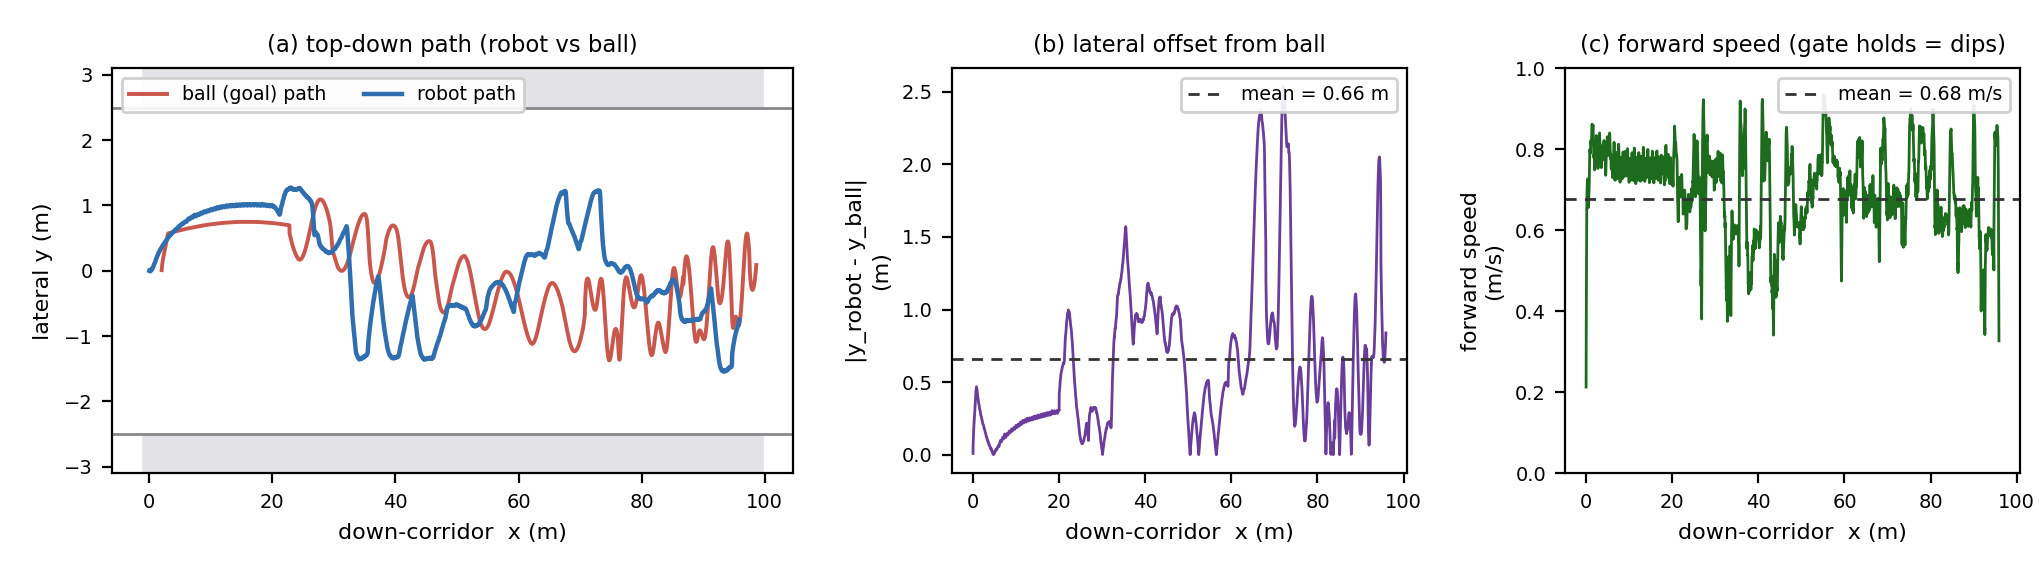
\includegraphics[width=\textwidth]{fig_trajectory.png}
\caption{One logged 150~s run (seed 42, collision-free). (a) Top-down paths: the robot
(blue) weaves its own route while the ball (red) walks its sine path through the obstacles;
grey bands are the corridor walls. (b) Lateral offset between robot and ball, mean 0.66~m.
(c) Forward speed; the dips are gate alignment holds.}
\label{fig:traj}
\end{figure*}

\textbf{Robustness.} To gauge how much the result leans on any single layer, we re-ran
three seeds at maximum difficulty (every lane at the 1.30~m floor) with parts of the stack
disabled. The robot stayed collision-free with the lateral-and-gate channel removed, and
again with the reactive avoidance removed (Table~\ref{tab:res}). We read this as defence in
depth: the guaranteed passable lane and the gap-steering planner already provide a safe
baseline, so no single layer is a single point of failure. What the lateral-and-gate channel
adds is precision rather than basic avoidance: with it on, the robot slows and centres
itself in each gap (the speed dips in Fig.~\ref{fig:traj}c) instead of cutting the corner;
with it off, the robot clears the same rows but tracks straighter and faster.

\begin{figure}[htbp]
\centering
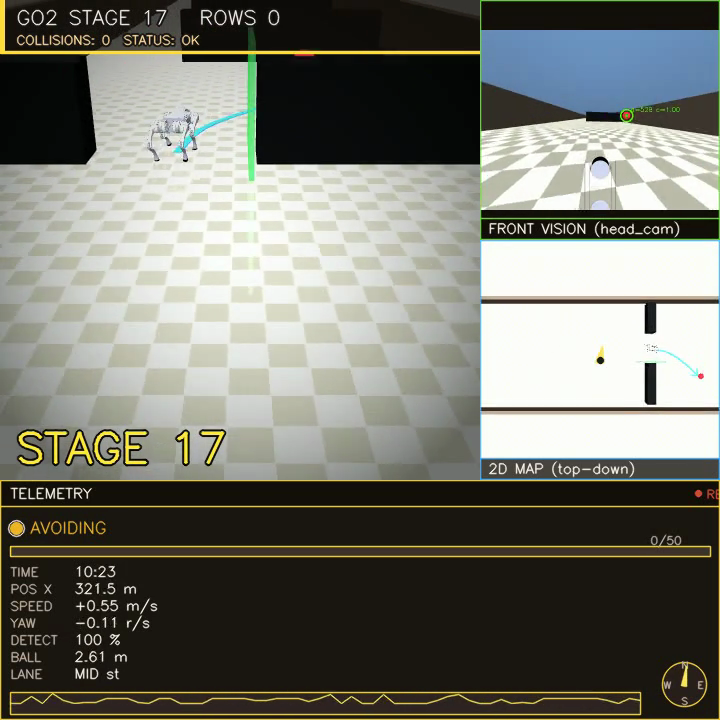
\includegraphics[width=\columnwidth]{fig_stage17.png}
\caption{Late in a run (stage 17, about 320~m in). Wide black obstacles fill the middle of
the corridor and the robot threads the lane that is left; the green halo marks the obstacle
being avoided, and the collision count is still zero.}
\label{fig:stage17}
\end{figure}

\section{Discussion and Limitations}
Two failure modes shaped the design. First, the original controller drove only forward
speed and yaw, so on a row whose only gap sat against a wall the robot could not line up
and clipped the obstacle. This pushed us to drive the sideways channel and add the gate.
Second, once the sideways channel was on, commanding a hard strafe and a hard turn
together built up enough roll to tip the robot over. We fixed this by shrinking the
sideways command during sharp turns and capping forward speed in that part of the policy's
command range. Both fixes are the lateral clip and the turn-rate guard of
Section~\ref{sec:vy}.

The walking policy is frozen and not fine-tuned for this task: it tracks sideways moves
with about 0.25~m of error and trips occasionally during the hardest cross-corridor moves.
We reduced both but did not remove them; the robot always recovered, and no trip became a
collision in the runs we report. Vision is colour-based, so a change in lighting or ball
colour would break it where a trained detector would not. Our evaluation covers a logged run
plus a three-seed ablation rather than an exhaustive sweep. Next steps are to fine-tune the
policy for tighter sideways tracking, replace the colour tracker with a learned detector,
and look one or two rows ahead so each gap is approached earlier.

\section{Conclusion}
A four-legged robot can cross a dense obstacle corridor collision-free --- to stage 17,
about 320~m, in a logged run --- using only a head camera and a walking policy it never
trained. Two changes made it work: drive the sideways velocity command the policy already
exposes, and refuse to enter a gap before lining up with it. A robustness check shows the system
leans on no single layer and degrades gracefully. The broader point is that extracting more
from a general pre-trained policy can stand in for a good deal of custom control and extra
sensing.

\begin{thebibliography}{9}
\bibitem{rudin} N. Rudin, D. Hoeller, P. Reist, and M. Hutter, ``Learning to Walk in
Minutes Using Massively Parallel Deep Reinforcement Learning,'' in \emph{Proc. CoRL},
2021. (source of our walking policy)
\bibitem{hwangbo} J. Hwangbo et al., ``Learning agile and dynamic motor skills for
legged robots,'' \emph{Science Robotics}, vol. 4, no. 26, 2019.
\bibitem{lee} J. Lee, J. Hwangbo, L. Wellhausen, V. Koltun, and M. Hutter, ``Learning
quadrupedal locomotion over challenging terrain,'' \emph{Science Robotics}, vol. 5,
no. 47, 2020.
\bibitem{coulter} R. C. Coulter, ``Implementation of the Pure Pursuit Path Tracking
Algorithm,'' Tech. Rep. CMU-RI-TR-92-01, Robotics Institute, Carnegie Mellon
University, 1992.
\bibitem{bradski} G. R. Bradski, ``Computer Vision Face Tracking for Use in a Perceptual
User Interface (CamShift),'' \emph{Intel Technology Journal}, 1998.
\bibitem{mujoco} E. Todorov, T. Erez, and Y. Tassa, ``MuJoCo: A physics engine for
model-based control,'' in \emph{Proc. IROS}, 2012.
\end{thebibliography}

\end{document}
